\section{Allgemeine Daten der Gebiete}
Wie in \autoref{sec:Vorgehensweise:Datendarstellung:Allgemeine Daten der Gebiete} beschrieben, werden zuerst allgemeine Daten der Landkreise und Regierungsbezirke ermittelt und dargestellt.
\section{Bevölkerungsdichten der Landkreise und Regierungsbezirke}
Die Landkreise in \autoref{fig:distribution_pop_density_counties} sind gemäß der Bevölkerungsdichte der Landkreise eingefärbt. Eine komplette Auflistung der Landkreise in dieser Reihenfolge findet sich in \autoref{tab:counties_by_pop_density}.
Klar zu erkennen die breite Spannweite von 35 bis 13~807 Einwohnern pro Quadratkilometer.

Aus der Auflistung in \autoref{tab:counties_by_pop_density} geht klar hervor, dass die 6 Gebiete mit der höchsten Bevölkerungsdichte die Bezirke Berlins sind. Rechnet man die Bevölkerungsdichte der gesamten Stadt Berlin zusammen, befindet sich diese auf Platz zwei und München besitzt mit 4765 Einwohnern pro Quadratkilometer die höchste Bevölkerungsdichte. 
\begin{figure}[H]
    \centering
    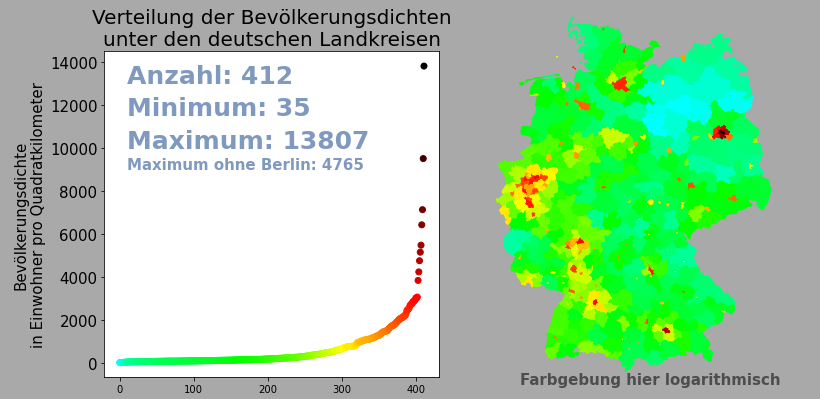
\includegraphics[width = \textwidth]{figures/Ergebnisse/population_density_counties.png}
    \caption{Verteilung der Bevölkerungsdichten der deutschen Landkreise $\rho_{\Omega}$, wie in \autoref{eq:Bevölkerungsdichte} beschrieben. Auf der linken Seite befindet sich die Verteilung, welche zudem die Farbgebung vorgibt. Auf der rechten Seite befindet sich die räumliche Anordnung. Die Farbgebung entspricht \autoref{sec:Grundlagen:Farbgebung}. Da jedoch wenige Werte sehr hoch sind, wie im linken Teil klar zu sehen, wird der Logarithmus der Bevölkerungsdichte benutzt, um die Farben zu vergeben.}
    \label{fig:distribution_pop_density_counties}
\end{figure}
\newpage
In \autoref{fig:distribution_pop_density_districts} sind die Bevölkerungsdichten der einzelnen Regierungsbezirke dargestellt. Wenig verwunderlich ist hier die Spannweite nicht ganz so groß: Die Auflistung der Regierungsbezirke nach Bevölkerungsdichte in \autoref{tab:districts_by_pop_density} beginnt mit Mecklenburg-Vorpommern (69.65 Einwohner pro Quadratkilometer) und endet mit Berlin (4107.70 Einwohner pro Quadratkilometer).

\begin{figure}[H]
    \centering
    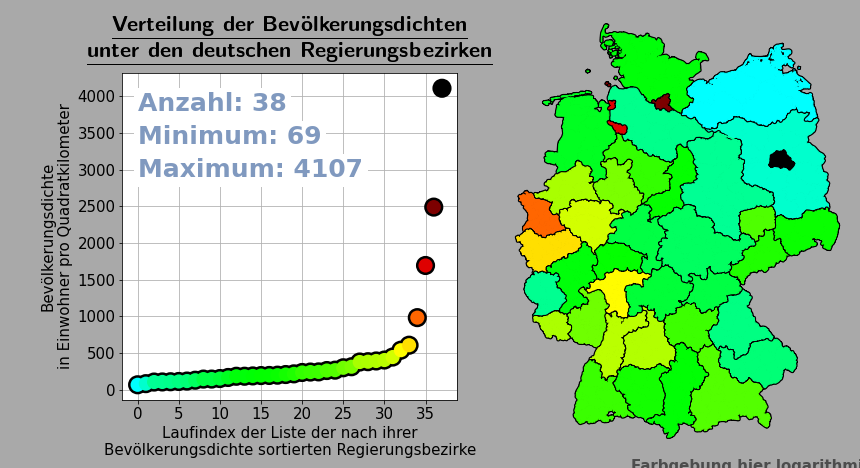
\includegraphics[width = \textwidth]{figures/Ergebnisse/population_density_ditricts.png}
    \caption{Verteilung der Bevölkerungsdichten der deutschen Regierungsbezirke $\rho_{\Omega}$, wie in \autoref{eq:Bevölkerungsdichte} beschrieben. Auf der linken Seite befindet sich die Verteilung, welche zudem die Farbgebung vorgibt. Auf der rechten Seite befindet sich die räumliche Anordnung. Die Farbgebung entspricht \autoref{sec:Grundlagen:Farbgebung}. Da jedoch wenige Werte sehr hoch sind, wie im linken Teil klar zu sehen, wird der Logarithmus der Bevölkerungsdichte benutzt, um die Farben zu vergeben.}
    \label{fig:distribution_pop_density_districts}
\end{figure}